\documentclass[11pt]{article}
\usepackage{textcomp,geometry,graphicx,verbatim}
\usepackage{fancyhdr}
\usepackage{amsmath,amssymb,enumerate,cancel}
\usepackage{titling}
\setlength{\droptitle}{-10em}   % This is your set screw
\pagestyle{fancy}
\def\Name{Manohar Jois}
\def\Homework{6} % Homework number - make sure to change for every homework!
\def\Session{Spring 2015}

% Extra commands
\let\origleft\left
\let\origright\right
\renewcommand{\left}{\mathopen{}\mathclose\bgroup\origleft}
\renewcommand{\right}{\aftergroup\egroup\origright}
\newcommand{\N}{\mathbb{N}}
\newcommand{\Z}{\mathbb{Z}}
\newcommand{\R}{\mathbb{R}}
\newcommand{\Q}{\mathbb{Q}}
\newcommand{\C}{\mathbb{C}}
\newcommand{\p}[1]{\left(#1\right)}
\newcommand{\E}{\mathbb{E}}
\newcommand{\cov}{\text{Cov}}
\newcommand{\deriv}[2]{\frac{d#1}{d#2}}
\newcommand{\pderiv}[2]{\frac{\partial#1}{\partial#2}}
\newcommand{\lhood}{\mathscr{L}}
\newcommand{\sig}[1]{\text{sig}\p{#1}}
\renewcommand{\gcd}[1]{\text{gcd}\p{#1}}
\renewcommand{\deg}[1]{\text{deg}\p{#1}}
\renewcommand{\log}[1]{\text{log}\p{#1}}
\renewcommand{\ln}[1]{\text{ln}\p{#1}}
\newcommand{\logb}[2]{\text{log}_{#1}\p{#2}}
\newcommand{\BigOh}[1]{O\p{#1}}
\newcommand{\BigOmega}[1]{\Omega\p{#1}}
\newcommand{\BigTheta}[1]{\Theta\p{#1}}
\newcommand{\asdf}{\newline\newline}

\title{CS189\ \Session\  --- Homework \Homework}
\author{\Name}
\lhead{CS189\ \Session\  Homework \Homework\ Problem \theproblemnumber,\ \Name}

\begin{document}
\maketitle
\newcounter{problemnumber}
\setcounter{problemnumber}{0}

\section*{Problem 1}
\stepcounter{problemnumber}
%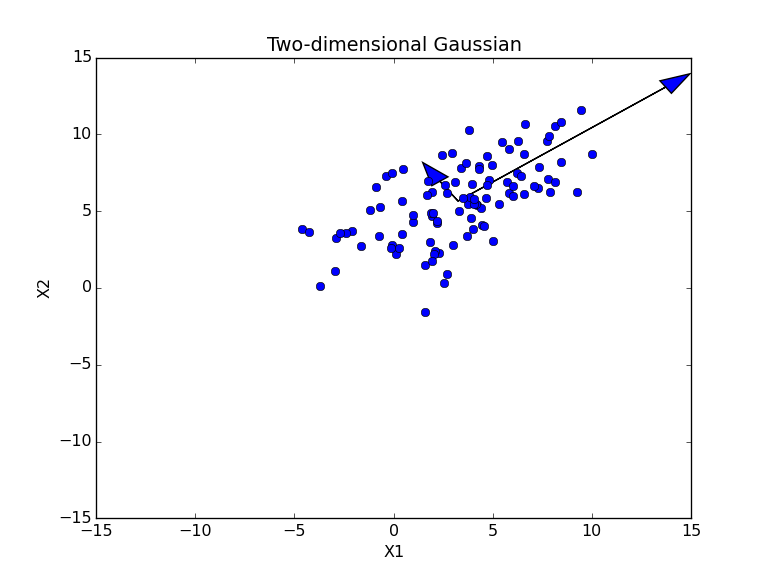
\includegraphics[scale=0.45]{images_hw3/p1d}
%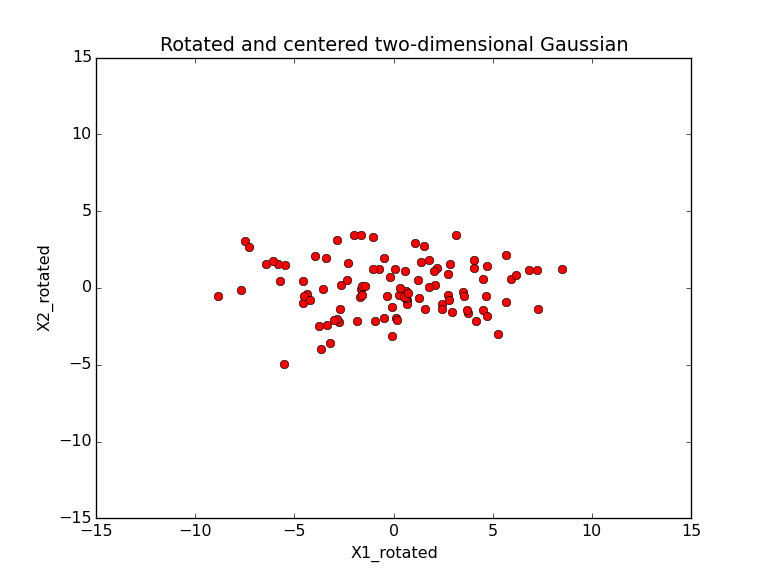
\includegraphics[scale=0.45]{images_hw3/p1e}
\begin{enumerate}[(1)]
\item We add the following notation:
\begin{itemize}
\item $n_i$ is the number of nodes in layer $i$.
\item $g_i(z)$ is the activation function for layer $i$, and "sig" is the sigmoid function.
\item $y$ is the $n_2\text{-by-}1$ vector of true labels (all zeros except one $1$).
\item $s^{(i)}$ is the $n_i\text{-by-}1$ input vector of layer $i$, in other words the weighted sum of the vector $x^{(i-1)}$.
\item $x^{(i)}$ is the $n_i\text{-by-}1$ activation output vector of layer $i$. Note that $W^{(i)T}x^{(i-1)}=s^{(i)}$ and $g_i(s^{(i)})=x^{(i)}$.
\item The symbol $\times$ represents element-wise multiplication, and fractions represent element-wise division.
\end{itemize}
\item Mean Squared Error
\begin{align*}
J &= \frac12(y-x^{(2)})^T(y-x^{(2)})\\
\pderiv J{W^{(2)}} &= \p{\p{\pderiv J{x^{(2)}}\times\pderiv {x^{(2)}}{s^{(2)}}}\p{\pderiv{s^{(2)}}{W^{(2)}}}^T}^T\qquad\text{(careful with dimensions)}\\
&= x^{(1)}\p{(y-x^{(2)})\times g_2'(s^{(2)})}^T\\
&= x^{(1)}\p{(y-x^{(2)})\times \sig{s^{(2)}}\times\p{1-\sig{s^{(2)}}}}^T\\
&= x^{(1)}\p{(y-x^{(2)})\times x^{(2)}\times\p{1-x^{(2)}}}^T\\
\pderiv J{W^{(1)}} &= \p{\pderiv J{s^{(1)}}\p{\pderiv{s^{(1)}}{W^{(1)}}}^T}^T\qquad\text{(careful with dimensions)}\\
&= x^{(0)}\p{\pderiv J{s^{(1)}}}^T\\
&= x^{(0)}\p{\pderiv{x^{(1)}}{s^{(1)}}\times \p{\pderiv{s^{(2)}}{x^{(1)}}\cdot \pderiv J{s^{(2)}}}}^T\qquad\text{(sum over all output nodes)}\\
&= x^{(0)}\p{g_1'\p{s^{(1)}}\times \p{W^{(2)}\cdot \pderiv J{s^{(2)}}}}^T\\
&= x^{(0)}\p{\p{1-\tanh^2\p{s^{(1)}}} \times \p{W^{(2)}\cdot \pderiv J{s^{(2)}}}}^T\\
&= x^{(0)}\p{\p{1-\p{x^{(1)}}^2} \times \p{W^{(2)}\cdot \pderiv J{s^{(2)}}}}^T\\
&= x^{(0)}\p{\p{1-\p{x^{(1)}}^2} \times \p{W^{(2)}\p{(y-x^{(2)})\times x^{(2)}\times\p{1-x^{(2)}}}}}^T
\end{align*}
\item Cross Entropy Error
\begin{align*}
J &= -\p{y\times\ln{x^{(2)}} + (1-y)\times\ln{1-x^{(2)}}}^T\p{y\times\ln{x^{(2)}} + (1-y)\times\ln{1-x^{(2)}}}\\
\pderiv J{x^{(2)}} &= -\p{\frac y{x^{(2)}} + \frac {1-y}{1-x^{(2)}}(-1)}\qquad\text{(element-wise derivative of sum of all elements)}\\
&= \p{\frac {1-y}{1-x^{(2)}} - \frac y{x^{(2)}}}\\
&= \frac{x^{(2)}-y}{x^{(2)}\times\p{1-x^{(2)}}}\\
\pderiv J{W^{(2)}} &= x^{(1)}\p{\pderiv J{x^{(2)}} \times g_2'(s^{(2)})}^T\\
&= x^{(1)}\p{\frac{x^{(2)}-y}{x^{(2)}\times\p{1-x^{(2)}}} \times x^{(2)}\times\p{1-x^{(2)}}}^T\\
&= x^{(1)}\p{x^{(2)}-y}^T\\
\pderiv J{W^{(1)}} &= x^{(0)}\p{g_1'\p{s^{(1)}}\times \p{W^{(2)}\cdot \pderiv J{s^{(2)}}}}^T\\
&= x^{(0)}\p{\p{1-\p{x^{(1)}}^2} \times \p{W^{(2)}\p{x^{(2)}-y}}}^T
\end{align*}
\item Stochastic gradient descent updates are the following for both loss metrics:
\begin{align*}
W^{(2)(t+1)} &\leftarrow W^{(2)(t)}-\eta\cdot\pderiv J{W^{(2)(t)}}\\
W^{(1)(t+1)} &\leftarrow W^{(1)(t)}-\eta\cdot\pderiv J{W^{(1)(t)}}
\end{align*}
\end{enumerate}


\newpage
\section*{Problem 2}
\stepcounter{problemnumber}
The weights were initialized from a Gaussian distribution with variance $\sigma^2=0.01$. The typical number of iterations run was $10^5$. In the plots below, the top row is MSE with $\eta=0.002$ and $79$ percent validation accuracy, while the bottom row is cross entropy with $\eta=0.0005$ and $81$ percent validation accuracy. Each took about $4$ minutes to train and calculate.\asdf
\begin{tabular}{cc}
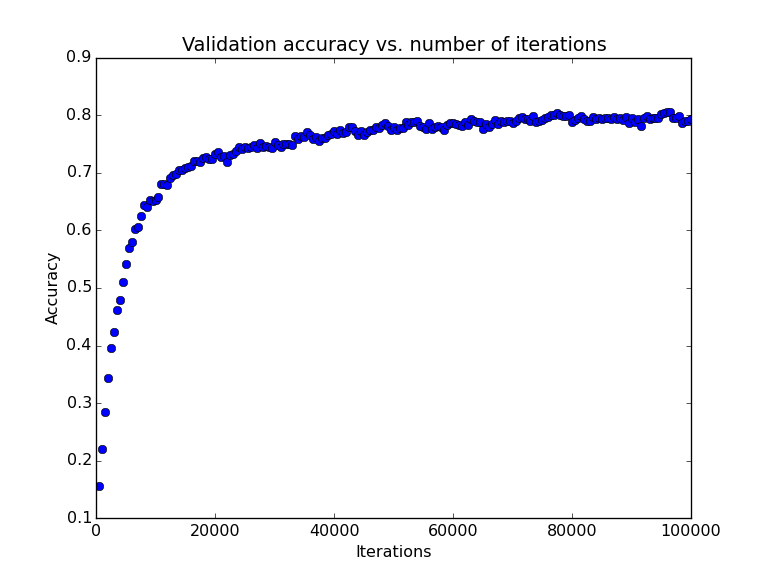
\includegraphics[scale=0.4]{images/accuracy_mse} & 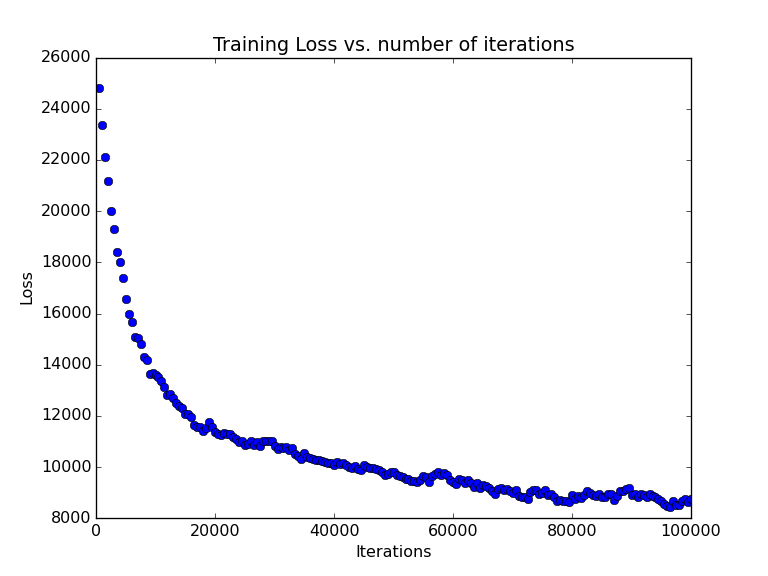
\includegraphics[scale=0.4]{images/loss_mse} \\
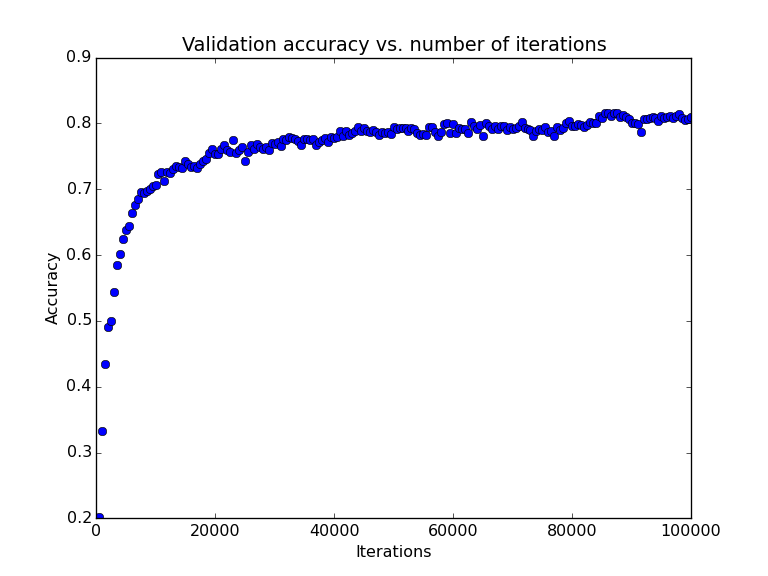
\includegraphics[scale=0.4]{images/accuracy_cross} & 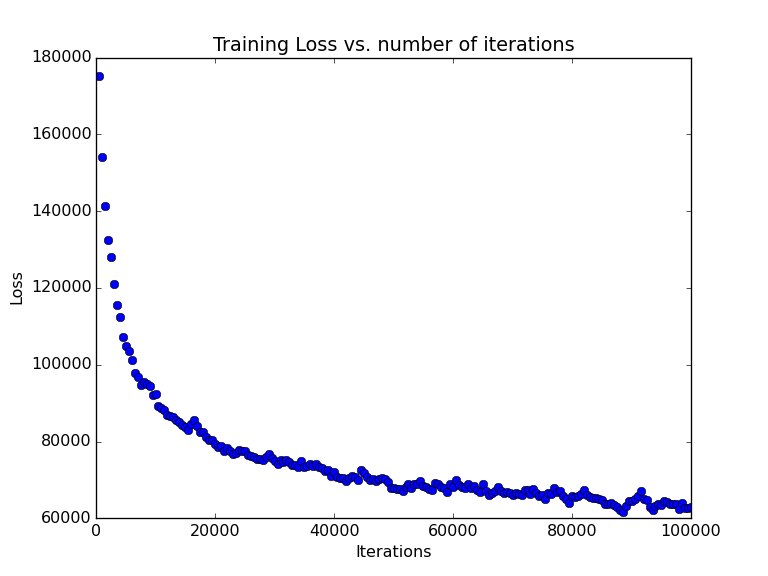
\includegraphics[scale=0.4]{images/loss_cross} \\
\end{tabular}\asdf
For Kaggle, I achieved just under $96$ percent accuracy with the same initialization, size-$2000$ mini-batch gradient descent, $10^4$ iterations and a learning rate of $10^{-4}$.\asdf
With the same number of iterations, cross entropy seems to perform slightly better in terms of both classification accuracy and training loss. It does require a smaller learning rate, which suggests the magnitude of the gradient with respect to the weights is larger and it doesn't find itself honing in on local minima throughout training.


\end{document}
